We introduce a system of parameters and constraints
to describe risk group turnover
in deterministic epidemic models with heterogeneity in risk.
We then describe how the system can be used in practical terms,
based on different assumptions and data available for parameterizing turnover in risk.
We conclude by framing previous approaches to this task using the proposed system.
% ==================================================================================================
\subsection{Notation}
\label{aa:notation}
Consider a population divided into $G$ risk groups.
We denote the number of individuals in risk group $i \in [1, \dots, G]$ as $x_i$
and the set of all risk groups as $\bm{x} = \{x_1, \dots, x_G\}$.
The total population size is $N = \sum_i {x_i}$,
and the relative population size of each group
is denoted as $\hat{x}_i = x_i / N$.
Individuals enter the population at a rate $\nu$ per year,
and exit at a rate $\mu$ per year.
We model the distribution of risk groups
among individuals entering into the population as $\bm{\hat{e}}$,
which may be different from individuals already in the population $\bm{\hat{x}}$.%
\footnote{We could equivalently stratify the rate of entry $\nu$ by risk group;
  however, we find that the mathematics in subsequent sections
  are more straightforward using $\bm{\hat{e}}$.}
Thus, the total number of individuals
entering into population $\bm{x}$ per year is given by $\nu N$,
and the number of individuals
entering into group $x_i$ specifically is given by $\hat{e}_i \nu N$.
% LW: I think the logic of this paragraph should be modified a bit.
%     When we say entry rate, we usually define it
%     from the perspective of the current population size (N).
%     So with an entry rate of v, and current population size of
%     N, the total number of individuals entering into population x per year is vN.
%     As u mentioned, we vN comes from e, which may have different risk group distribution,
%     and the number of individuals entering into group x_i can thus be given by ê_i ν N.
%     Up till here, it is all independent of our assumption that e has size of N.
%     Risk groups, transitions, and the associated rates are also shown for G = 3 in Figure 1.
%     We assume that population e also has size N given the rational u described here.
%     That way, the number of individuals entering into group
%     x_i specifically is given by e_i ν.
% JK: Is this better?
\par
Turnover transitions may then occur between any two groups, in either direction.
Therefore we denote the turnover rates as a $G \times G$ matrix $\phi$.
The element $\phi_{ij}$ corresponds to the proportion of individuals in group $x_i$
who move from group $x_i$ to group $x_j$ each year.
An example matrix is given in Eq.~(\ref{eq:phi}),
where we write the diagonal elements as $*$ since they represent
transitions from a group to itself.
\begin{equation}\label{eq:phi}
\phi = \left[\begin{array}{cccc}
	         *          & x_1  \rightarrow x_2 & \cdots & x_1 \rightarrow x_G \\[0.5em]
	x_2 \rightarrow x_1 &          *           & \cdots & x_2 \rightarrow x_G \\[0.5em]
	      \vdots        &        \vdots        & \ddots &       \vdots        \\[0.5em]
	x_G \rightarrow x_1 & x_G \rightarrow x_2  & \cdots &          *
\end{array}\right]
\end{equation}
Risk groups, transitions, and the associated rates
are also shown for $G = 3$ in Figure~\ref{fig:system-app}.
\begin{figure}
  \centering
  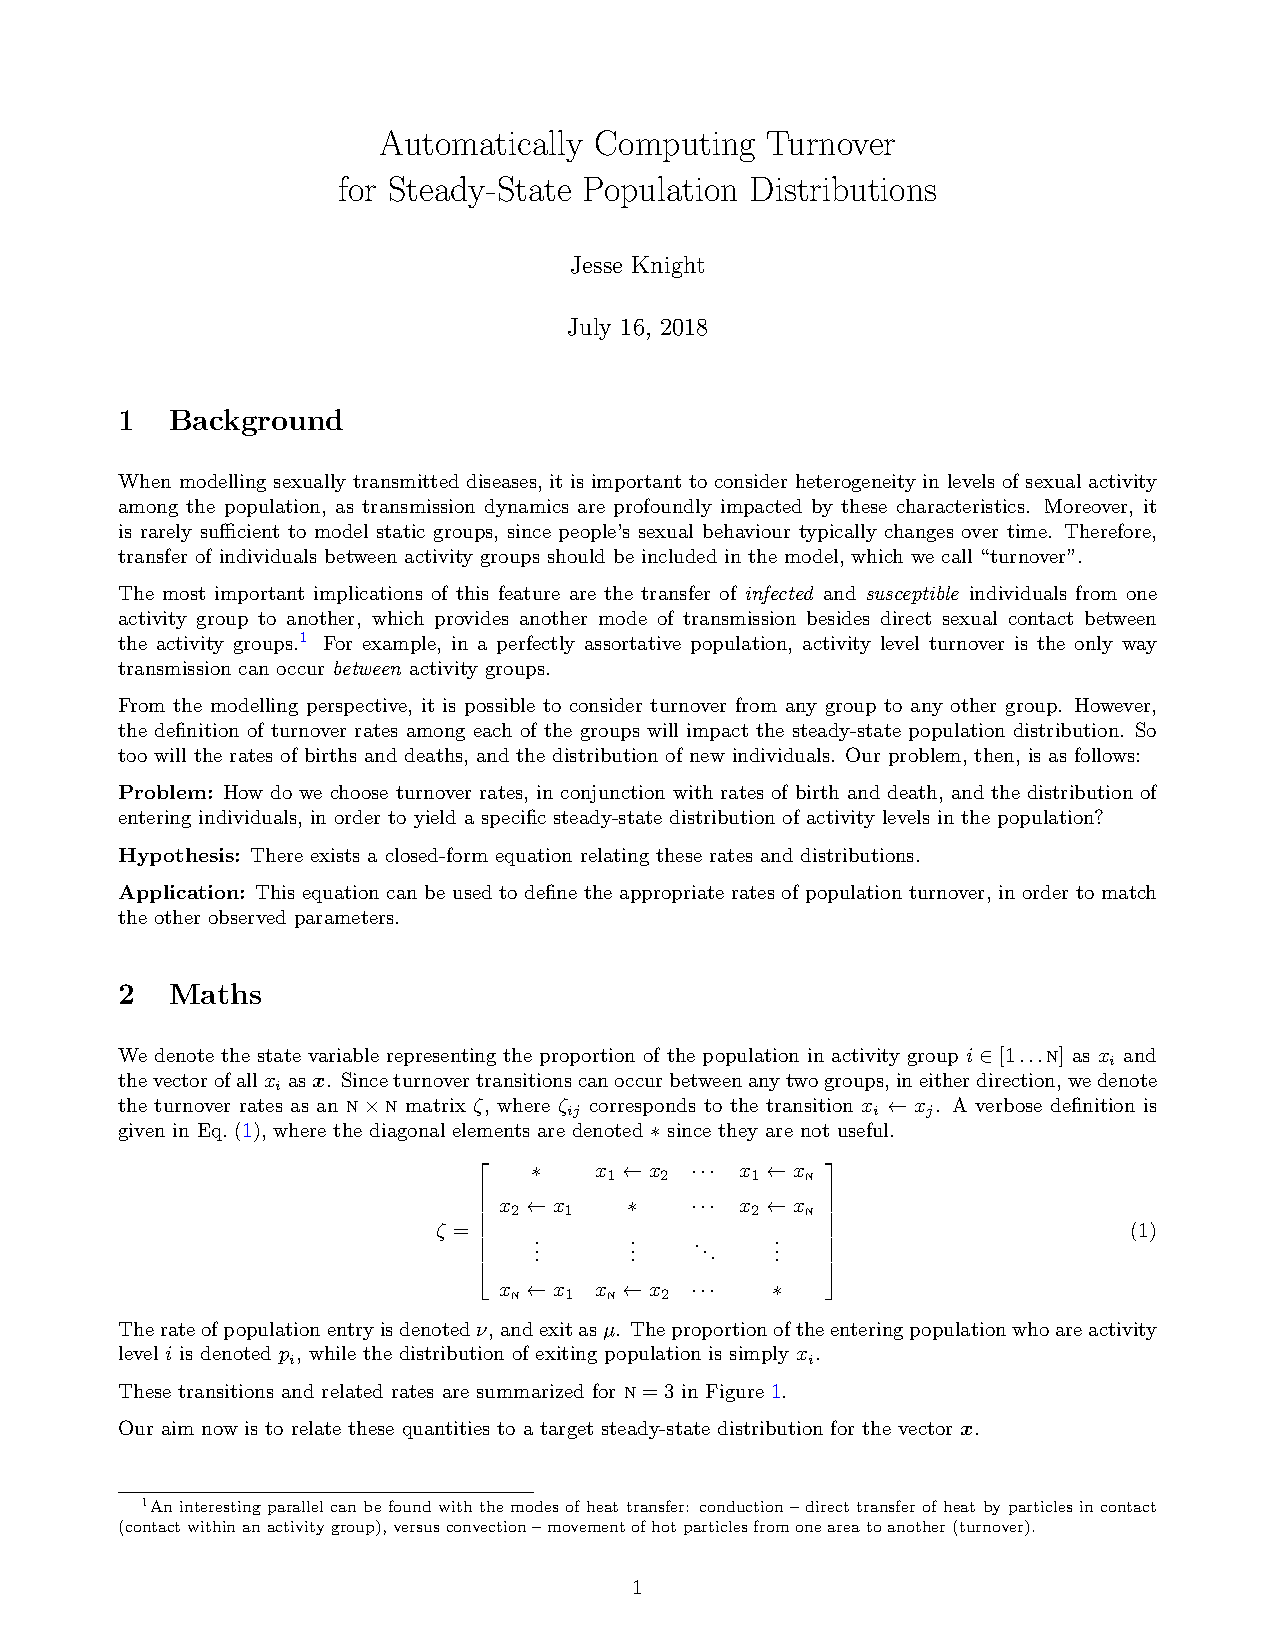
\includegraphics[width=0.5\linewidth]{turnover}
  \caption{System of risk groups and flows between them for $G = 3$}
  \label{fig:system-app}
\end{figure}
% ==================================================================================================
\subsection{Parameterization}
\label{aa:params}
Next, we construct a system like the one above
which reflects the risk group dynamics observed in a specific context.
We assume that the relative sizes of the risk groups in the model ($\bm{\hat{x}}$)
are already known, and should remain constant over time.
Thus, what remains is to estimate the values of the parameters:
$\nu$, $\mu$, $\bm{\hat{e}}$, and $\phi$,
using commonly available sources of data.
% --------------------------------------------------------------------------------------------------
\subsubsection{Total Population Size}
\label{aaa:params-nu-mu}
The total population size $N(t)$ is a function of
the rates of population entry $\nu(t)$ and exit $\mu(t)$, given an initial size $N_0$.
We allow the proportion entering the system to vary by risk group via $\bm{\hat{e}}$,
while the exit rate has the same value for each group.
We assume that there is no disease-attributable death.
Because the values of $\nu$ and $\mu$ are the same for each risk group, 
they can be estimated independent of
$\bm{\hat{x}}$, $\bm{\hat{e}}$, and $\phi$.
\par
The difference between entry and exit rates
defines the rate of population growth:
\begin{equation}\label{eq:growth-G}
\mathcal{G}(t) = \nu(t) - \mu(t) 
\end{equation}
The total population may then be defined using an initial population size $N_0$ as:
\begin{equation}\label{eq:growth-vary}
N(t) = N_0 \exp{\left(\int_{0}^{\,t}{\log\big(1+\mathcal{G}(\tau) \big)d\tau}\right)}
\end{equation}
which, for constant growth, simplifies to the familiar expression~\citep{Malthus1798}:
\begin{equation}\label{eq:growth-const}
N(t) = N_0 {(1 + \mathcal{G})}^{t}
\end{equation}
Census data, such as \citep{WorldBank}, can be used to source
the total population size in a given geographic setting over time $N(t)$,
thus allowing Eqs.~(\ref{eq:growth-vary})~and~(\ref{eq:growth-const})
to be used to estimate $\mathcal{G}(t)$.
\par
If the population size is assumed to be constant,
then $\mathcal{G}(t) = 0$ and $\nu(t) = \mu(t)$.
If population growth occurs at a stable rate, then
$\mathcal{G}$ is fixed at a constant value
which can be estimated via Eq.~(\ref{eq:growth-const})
using any two values of $N(t)$, separated by a time interval $\tau$:
\begin{equation}\label{eq:growth-backwards}
\mathcal{G}_{\tau} = {\frac{N(t+\tau)}{N(t)}}^{\frac{1}{\tau}} -1
\end{equation}
If the rate of population growth $\mathcal{G}$ varies over time,
then Eq.~(\ref{eq:growth-backwards}) can be reused for consecutive time intervals,
and the complete function $\mathcal{G}(t)$ approximated piecewise by constant values.
The piecewise approximation can be more feasible
than exact solutions using Eq.~(\ref{eq:growth-vary}),
and can reproduce $N(t)$ accurately for small enough intervals $\tau$,
such as one year.
\par
Now, given a value of $\mathcal{G}(t)$,
either $\nu(t)$ must be chosen and $\mu(t)$ calculated using Eq.~(\ref{eq:growth-G}),
or $\mu(t)$ must be chosen, and $\nu(t)$ calculated.
Most modelled systems assume
a constant duration of time that individuals spend in the model $\delta(t)$~\citep{Anderson1991}
which is related to the rate of exit $\mu$ by:
\begin{equation}\label{eq:duration-model}
\delta(t) = \mu^{-1}(t)
\end{equation}
In the context of sexually transmitted infections, the duration of time usually reflects
the average sexual life-course of individuals from age 15~to~50 years,
such that $\delta = 35$ years.
The duration $\delta$ may also vary with time to reflect changes in life expectancy.
The exit rate $\mu(t)$ can then be defined as $\delta^{-t}(t)$
following Eq.~(\ref{eq:duration-model}),
and the entry rate $\nu(t)$ defined as $\mathcal{G}(t) - \mu(t)$
following Eq.~(\ref{eq:growth-G}).
% --------------------------------------------------------------------------------------------------
\subsubsection{Turnover}
\label{aaa:params-turnover}
Next, we present methods for resolving
the distribution of individuals entering the risk model $\bm{\hat{e}}(t)$ and
the rates of turnover $\phi(t)$,
assuming that entry and exit rates $\nu(t)$ and $\mu(t)$ are known.
Similar to above, we first formulate the problem as a system of equations.
Then, we explore the data and assumptions required
to solve for the values of parameters in the system.
The $(t)$ notation is omitted throughout this section for clarity,
though time-varying parameters can be estimated by
repeating the necessary calculations for each $t$.
\par
The number of risk groups $G$ dictates the number of
unknown elements in $\bm{\hat{e}}$ and $\phi$: $G$ and $G(G-1)$, respectively.
We collect these unknowns in the vector
$\bm{\theta} = \left[\bm{\hat{e}}, \bm{y}\right]$,
where $\bm{y} = \mathrm{vec}_{i \ne j}(\phi)$.
For example, for $G = 3$, the vector $\bm{\theta}$ is defined as:
\begin{equation}
\bm{\theta} = \left[
\begin{array}{ccccccccc}
\hat{e}_1 & \hat{e}_2 & \hat{e}_3 & \phi_{12} & \phi_{13} & \phi_{21} & \phi_{23} & \phi_{31} & \phi_{32}
\end{array}\right]
\end{equation}
We then define a linear system of equations
which uniquely determine the elements of $\bm{\theta}$:
\begin{equation}\label{eq:system-matrix-app}
\bm{b} = A \thinspace \bm{\theta}
\end{equation}
where $A$ is a $M \times G^2$ matrix
and $\bm{b}$ is a $M$-length vector.
Specifically, each row in $A$ and $\bm{b}$ defines a constraint:
an assumed mathematical relationship involving one or more elements of
$\bm{\hat{e}}$ and $\phi$.
For example, a simple constraint could be to assume the value $\hat{e}_2 = 0.20$.
Each of the following sections introduces a type of constraint, including:
assuming a constant group size,
specifying elements of $\bm{\theta}$ directly,
assuming an average duration in a group,
and assuming relative rates of turnover.
Constraints may be selected and combined together based on
availability of data and plausibility of assumptions.
However, a total of $M = G^2$ constraints must be defined
in order to obtain a ``unique solution'':
exactly one value of $\bm{\theta}$ which satisfies all constraints.
The values of $\bm{\hat{e}}$ and $\phi$
can then be calculated algebraically by solving Eq.~(\ref{eq:system-matrix-app})
with $\bm{\theta} = A^{-1}\bm{b}$,
for which many algorithms exist~\citep{LAPACK}.
% --------------------------------------------------------------------------------------------------
\paragraph{1.~Constant group size}
\label{con:const-group}
One epidemiologic feature that epidemic models consider
is whether or not the relative sizes of risk groups are constant over time
\citep{Henry2015,Boily2015}.
Assuming constant group size implies a stable level of heterogeneity over time.
To enforce this assumption,
we define the ``conservation of mass'' equation for group $x_i$,
wherein the rate of change of the group
is defined as the sum of flows in\,/\,out of the group:
\begin{equation}\label{eq:mass-balance-1}
\frac{d}{dt}x_i
= \nu N \hat{e}_i + \sum_{j}{\phi_{ji} \thinspace x_j}
- \mu \thinspace x_i - \sum_{j}{\phi_{ij} \thinspace x_i}
\end{equation}
Eq.~(\ref{eq:mass-balance-1}) is written in terms of
absolute population sizes $\bm{x}$,
but can be written as proportions $\bm{\hat{x}}$
by dividing all terms by $N$.
If we assume that the proportion of each group $\hat{x}_i$ is constant over time,
then the desired rate of change for risk group $i$
will be equal to the rate of population growth of the risk group, $\mathcal{G} x_i$.
Substituting $\frac{d}{dt}x_i = \mathcal{G} x_i$
into Eq.~(\ref{eq:mass-balance-1}),
and simplifying yields:
\begin{equation}\label{eq:mass-balance-2}
\nu \thinspace x_i
= \nu \thinspace N \hat{e}_i + \sum_{j}{\phi_{ji} \thinspace x_j}
- \sum_{j}{\phi_{ij} \thinspace x_i}
\end{equation}
Factoring the left and right hand sides in terms of $\bm{\hat{e}}$ and $\phi$,
we obtain $G$ unique constraints.
For $G = 3$, this yields the following 3 rows as the basis of $\bm{b}$ and $A$:
\begin{equation}\label{eq:eg-basis}
\bm{b} = \left[\begin{array}{c}
\nu x_1 \\ \nu x_2 \\ \nu x_3
\end{array}\right];\qquad
A = \left[\begin{array}{ccccccccc}
	 \nu  & \cdot & \cdot & -x_1  & -x_1  &  x_2  & \cdot &  x_3  & \cdot \\
	\cdot &  \nu  & \cdot &  x_1  & \cdot & -x_2  & -x_2  & \cdot &  x_3  \\
	\cdot & \cdot &  \nu  & \cdot &  x_1  & \cdot &  x_2  & -x_3  & -x_3
\end{array}\right] 
\end{equation}
These $G$ constraints ensure risk groups do not change size over time.
However, a unique solution requires
an additional $G(G-1)$ constraints.
For $G = 3$, this corresponds to 6 additional constraints.
% --------------------------------------------------------------------------------------------------
\paragraph{2.~Specified elements}
\label{con:spec-element}
The simplest type of additional constraint is to
directly specify the values of individual elements in $\bm{\hat{e}}$ or $\phi$.
Such constraints may be appended to $\bm{b}$ and $A$
as an additional row $k$ using indicator notation.%
\footnote{Indicator notation, also known as ``one-hot notation'' is used to
  select one element from another vector, based on its position.
  An indicator vector is 1 in the same location as the element of interest,
  and 0 everywhere else.}
That is, with $b_k$ as the specified value $v$,
and $A_k$ as the indicator vector,
with $1$ in the same position as the desired element in $\bm{\theta}$:
\begin{equation}\label{eq:spec-elem}
b_k = v;\qquad
A_k = [0,\dots,1,\dots,0]
\end{equation}
For example, for $G = 3$, if it is known that 20\% of individuals
enter directly into risk group $x_2$ upon entry into the model ($\hat{e}_2 = 0.20$),
then $\bm{b}$ and $A$ can be augmented with:
\begin{equation}\label{eq:eg-spec}
b_k = \left[\begin{array}{c} 0.20 \end{array}\right];\qquad
A_k = \left[\begin{array}{ccccccccc}
	\cdot & 1 & \cdot & \cdot & \cdot & \cdot & \cdot & \cdot & \cdot
\end{array}\right] 
\end{equation}
since $\hat{e}_2$ is the second element in $\bm{\theta}$.
If the data suggest zero turnover from group $i$ to group $j$,
then Eq.~(\ref{eq:eg-spec}) can also be used to set $\phi_{ij} = 0$.
\par
Note that the elements of $\bm{\hat{e}}$ must sum to one.
Therefore, specifying all elements in $\bm{\hat{e}}$
will only provide $G-1$ constraints,
as the last element will be either redundant or violate the sum-to-one rule.
As shown in Appendix~\ref{aa:eqs-e-redundant},
the sum-to-one rule is actually implicit in Eq.~(\ref{eq:eg-basis}),
so it is not necessary to supply a constraint like $1 = \sum_{i} \hat{e}_i$.
% --------------------------------------------------------------------------------------------------
\paragraph{3.~Group duration}
\label{con:group-dur}
Type 1 Constraints assume that the relative population size of each group remains constant.
Another epidemiologic feature that epidemic models considered
is whether or not the duration of time spent within a given risk group remains constant.
For example, in STI transmission models that include formal sex work,
it can be assumed that the duration in formal sex work work remains stable over time,
such as in \citep{Mishra2014a,Boily2015}.
The duration $\delta_i$ is defined as the inverse of all rates of exit from the group:
\begin{equation}\label{eq:duration-group}
\delta_i = {\bigg(\mu + \sum_{j}{\phi_{ij}}\bigg)}^{-1}
\end{equation}
Estimates of the duration in a given group can be sourced from
cross-sectional survey data where participants are asked about
how long they have engaged in a particular practice
-- such as sex in exchange for money \citep{Watts2010}.
Data on duration may also be sourced from longitudinal data,
where repeated measures of self-reported sexual behaviour,
or proxy measures of sexual risk data,
are collected \citep{DHS,PHIAproject}.
Data on duration in each risk group can then be used to define $\phi$ by
rearranging Eq.~(\ref{eq:duration-group}) to yield:
${\delta_{i}}^{-1} - \mu = \sum_{j}{\phi_{ij}}$.
For example, if for $G = 3$,
the average duration in group $x_1$ is known to be $\delta_1 = 5$ years,
then $\bm{b}$ and $A$ can be augmented with another row $k$:
\begin{equation}\label{eq:eg-dur}
b_k = \left[\begin{array}{c}
{5}^{-1} - \mu
\end{array}\right];\qquad
A_k = \left[\begin{array}{ccccccccc}
	\cdot & \cdot & \cdot & 1 & 1 & \cdot & \cdot & \cdot & \cdot
\end{array}\right]
\end{equation}
\par
Note that, similar to specifying all elements of $\bm{\hat{e}}$,
specifying $\delta_i$ may result in conflicts or redundancies with other constraints.
A conflict means it will not be possible to resolve values of $\phi$
which simultaneously satisfy all constraints, while
a redundancy means that adding one constraint does not help resolve
a unique set of values $\bm{\theta}$.
For example, for $G = 3$,
if Type 2 Constraints are used to specify $\phi_{12} = 0.1$ and $\phi_{13} = 0.1$,
and $\mu = 0.05$, then by Eq.~(\ref{eq:duration-group}), we must have
$\delta_1 = 4$.
Specifying any other value for $\delta_1$ will result in a conflict,
while specifying $\delta_1 = 4$ is redundant,
since it is already implied.
There are innumerable situations in which this may occur,
so we do not attempt to describe them all.
Section~\ref{p:solving} describes how to identify
conflicts and redundancies when they are not obvious.
% --------------------------------------------------------------------------------------------------
\paragraph{4.~Turnover rate ratios}
\label{con:rel-turnover}
In many cases, it may be difficult to
obtain estimates of a given turnover rate $\phi_{ij}$
for use in Type 2 Constraints.
However, it may be possible to estimate
relative relationships between rates of turnover,
such as:
\begin{equation}\label{eq:ratio}
r\,\phi_{ij} = \phi_{i'j'}
\end{equation}
where $r$ is a ratio relating the values of $\phi_{ij}$ and $\phi_{i'j'}$.
For example, for $G = 3$,
let $T_1$ be the total number of individuals entering group $x_1$ due to turnover.
If we know that
70\% of $T_1$ originates from group $x_2$, while
30\% of $T_1$ originates from group $x_3$,
then $0.7\,T_1 = \phi_{23} \, x_2$ and $0.3\,T_1 = \phi_{13} \, x_1$,
and thus: $\phi_{23} \left(\frac{0.3\,x_2}{0.7\,x_1}\right) = \phi_{13}$.
This constraint can then be appended as another row $k$ in $\bm{b}$ and $A$ like:
\begin{equation}\label{eq:eg-ratio}
b_k = \left[\begin{array}{c}
0
\end{array}\right];\qquad
A_k = \left[\begin{array}{ccccccccc}
	\cdot & \cdot & \cdot & \cdot & \left(\frac{0.3\,x_2}{0.7\,x_1}\right) & \cdot & 1 & \cdot & \cdot
\end{array}\right] 
\end{equation}
The example in Eq.~(\ref{eq:eg-ratio}) is based on
what proportions of individuals entering a risk group $j$
came from which former risk group $i$,
but similar constraints may be defined based on
what proportions of individuals exiting a risk group $i$
enter into which new risk group $j$.
It can also be assumed that
the absolute number of individuals moving between two risk groups is equal,
in which case the relationship is:
$\phi_{ij} \left(\frac{x_i}{x_j}\right) = \phi_{ji}$.
All constraints of this type will have $b_k = 0$.
% --------------------------------------------------------------------------------------------------
\paragraph{Solving the System}
\label{p:solving}
Table~\ref{tab:constraints-app} summarizes the four types of constraints described above.
Given a set of sufficient constraints on $\bm{\theta}$
to ensure exactly one solution, the system of equations Eq.~(\ref{eq:system-matrix-app})
can be solved using $\bm{\theta} = A^{-1}\bm{b}$.
The resulting values of $\bm{\hat{e}}$ and $\phi$ can then be used
in the epidemic model.
\par
However, we may find that we have an insufficient number of constraints, implying that
there are multiple values of the vector $\bm{\theta}$ which satisfy the constraints.
An insufficient number of constraints may be identified
by a ``rank deficiency'' warning
in numerical solvers of Eq.~(\ref{eq:system-matrix-app}) \citep{LAPACK}.
Even if $A$ has $G^2$ rows,
the system may have an insufficient number of constraints
because some constraints are redundant.
In this situation, we can pose the problem as a minimization problem, namely:
\begin{equation}\label{eq:system-optimize}
\bm{\theta}^{*} = {\arg \min}
\thinspace f(\bm{\theta}),
\quad \textrm{subject to:}
\enspace\bm{b} = A\thinspace\bm{\theta};
\enspace\bm{\theta} \ge 0
\end{equation}
where $f$ is a function which penalizes certain values of $\bm{\theta}$.
For example, $f = {\left|\left| \,\cdot\, \right|\right|}_2$
penalizes large values in $\bm{\theta}$,
so that the smallest values of $\bm{\hat{e}}$ and $\phi$
which satisfy the constraints will be resolved.%
\footnote{Numerical solutions to such problems are widely available,
  such as the Non-Negative Lease Squares solver \citep{Lawson1995},
  available in Python:
  \href{https://docs.scipy.org/doc/scipy/reference/generated/scipy.optimize.nnls.html}
  {\texttt{https://docs.scipy.org/doc/scipy/reference/generated/scipy.optimize.nnls.html}}.}
\par
Similarly, we may find that no solution exists for the given constraints,
since two or more constraints are in conflict.
Conflicting constraints may be identified by a non-zero error
in the solution to Eq.~(\ref{eq:system-matrix-app}) \citep{LAPACK}.
In this case, the conflict should be resolved by
changing or removing one of the conflicting constraints.
\begin{table}
  \centering
  \caption{Summary of constraint types for defining risk group turnover}
  \label{tab:constraints-app}
  \begin{tabular}{lccl}
	\toprule
	Name                    &            Eq.            &        E.g.         & Data requirements                                                         \\
	\midrule
	1.~Constant group size  & (\ref{eq:mass-balance-2}) & (\ref{eq:eg-basis}) & all values of $\hat{x}_i$ and $\nu$                                       \\
	2.~Specified elements   &   (\ref{eq:spec-elem})    & (\ref{eq:eg-spec})  & any value of $\hat{e}_i$ or $\phi_{ij}$                                   \\
	3.~Group duration       & (\ref{eq:duration-group}) &  (\ref{eq:eg-dur})  & any value of $\delta_i$                                                   \\
	4.~Turnover rate ratios &     (\ref{eq:ratio})      & (\ref{eq:eg-ratio}) & any relationship between two turnover rates $\phi_{ij}$ and $\phi_{i'j'}$ \\
	\bottomrule
\end{tabular}\\[1em]
\footnotesize\flushleft
$\nu$:~rate of population entry;
$\phi_{ij}$:~rate of turnover from group $i$ to group $j$;
$\hat{x}_i$:~proportion of individuals in risk group $i$;
$\hat{e}_i$:~proportion of individuals entering into risk group $i$;
$\delta_i$:~average duration spent in risk group $i$.
\end{table}
% ==================================================================================================
\subsection{Previous Approaches}
\label{aa:prev-appr}
Few epidemic models of sexually transmitted infections
with heterogeneity in risk
have simulated turnover among risk groups,
and those models which have simulated turnover
have done so in various ways.
In this section, we review
three prior implementations of turnover and each study's objectives for the implementation
-- e.g. constant relative group sizes over time.
We then highlight how the approach proposed in Section~\ref{aa:params}
could be used to achieve the same objectives.
% --------------------------------------------------------------------------------------------------
\par
\citet{Stigum1994} simulated turnover among $G = 2$ risk groups
in a population with no exogenous entry or exit
($\nu = \mu = 0$ and hence $\bm{\hat{e}}$ is not applicable).
Turnover between the groups was balanced
in order to maintain constant risk group sizes (Type 1 Constraint),%
\footnote{Due to its simplicity,
  this constraint is actually an example of both Type 1 and Type 4 Constraints.}
while the rate of turnover from high to low
was specified as $\kappa$ (Type 2 Constraint).
Thus, the turnover system used by \citet{Stigum1994} can be written
in the proposed framework as:
\begin{equation}\label{eq:sys-Stigum1994}
\left[\begin{array}{c}
    0    \\
  \kappa
\end{array}\right]
=
\left[\begin{array}{cc}
  \hat{x}_1 & -\hat{x}_2 \\
      1     &   \cdot
\end{array}\right]
\left[\begin{array}{c}
  \phi_{12} \\
  \phi_{21}
\end{array}\right]
,\qquad
\hat{e}_1 = \hat{e}_2 = 0
\end{equation}
% --------------------------------------------------------------------------------------------------
\par
\citet{Henry2015} also simulated turnover among $G = 2$ risk groups,
but considered exogenous entry and exit, both at a rate $\mu$.
The authors used the notation $f_i$ for our $\hat{x}_i$, and assumed that
the exogenous population had the same distribution of risk groups
as the system population: $\hat{e}_i = f_i$ (Type 2 Constraint).
The authors further maintained constant risk group sizes (Type 1 Constraint)
by analytically balancing turnover between the two groups using:
$\phi_{12} = \omega \hat{x}_2 ;\enspace \phi_{21} = \omega \hat{x}_1$.
However, it can be shown that this analytical approach
is also the solution to the following combination of Type 1 and 2 Constraints:
\begin{equation}\label{eq:sys-Henry2015}
\left[\begin{array}{c}
      0      \\
  \omega f_2
\end{array}\right]
=
\left[\begin{array}{cc}
  f_1 & -f_2  \\
   1  & \cdot
\end{array}\right]
\left[\begin{array}{c}
  \phi_{12} \\
  \phi_{21}
\end{array}\right]
,\qquad
\hat{e}_i = f_i
\end{equation}
% --------------------------------------------------------------------------------------------------
\par
\citet{Eaton2014} simulated turnover among $G = 3$ risk groups,
considering exogenous entry from a population
with a unique distribution of risk groups $\bm{\hat{e}}$.
Turnover was considered from
high-to-medium, high-to-low, and medium-to-low risk,
all with an equal rate $\psi$;
the reverse transition rates were set to zero
(six total Type 2 Constraints).
In the absence of turnover in the other direction,
risk group sizes were maintained using the values of $\hat{e}_i$,
computed using Type 1 Constraints as follows:
\begin{equation}\label{eq:sys-Eaton2014-simple}
\left[\begin{array}{l}
\nu x_1 + 2 x_1 \psi \\
\nu x_2 -   x_1 \psi + x_2 \psi \\
\nu x_3 -   x_1 \psi - x_2 \psi
\end{array}\right]
=
\left[\begin{array}{ccc}
\nu  & \cdot & \cdot \\
\cdot &  \nu  & \cdot \\
\cdot & \cdot &  \nu  \\
\end{array}\right]
\left[\begin{array}{c}
e_1 \\
e_2 \\
e_3
\end{array}\right]
,\qquad
\begin{array}{c}
\phi_{12} = \phi_{13} = \phi_{23} = \psi\\
\phi_{21} = \phi_{31} = \phi_{32} = 0
\end{array}
\end{equation}

% --------------------------------------------------------------------------------------------------
\par
In sum, the framework for modelling turnover presented in this section
aims to generalize all previous implementations.
In so doing, we hope to clarify the requisite assumptions,
dependencies on epidemiologic data,
and relationships between previous approaches.
